\section{Herkunft des Saga-Patterns}\label{sec:section-garcia-paper}

Das Implementierungsmuster einer Saga stammt aus dem \citeyear{GarciaMolina.1987} veröffentlichten Paper \citetitle{GarciaMolina.1987}. Darin adressieren \citeauthor{GarciaMolina.1987} die blockierende Eigenschaft von \acrfull{llt} und führen das Sagamuster als Problemlösung ein. 

\subsection{Langlebige Transaktionen}
Damit die transaktionelle Implementierung eines Prozesses die ACID-Eigenschaften gewährleisten kann, werden Datenbanksperren verwendet. Ein solcher Lock sperrt ausgewählte Ressourcen für die Dauer der Transaktion. Eine LLT repräsentiert einen solchen transaktionellen Prozess, der eine sehr hohe Ausführungsdauer hat. Als Ursache für diese lange Dauer nennen \citeauthor{GarciaMolina.1987} viele langwierige Berechnungsschritte und die Pausierung zum Warten auf Benutzerinput \citep[p.~1]{GarciaMolina.1987}. 

\subsection{Auftrennung einer LLT in Teiltransaktionen}
Als Lösung für die blockierende Eigenschaft von LLT formulieren \citeauthor{GarciaMolina.1987} das Saga-Pattern, welches die Atomarität eines transaktionellen Prozesses auflöst und die LLT per Teiltransaktionen realisiert. Die LLT wird in kleinere Teiltransaktionen aufgebrochen und sequentiell durchgeführt. Jedes T wird dabei mit einer zugehörigen kompensierenden Transaktion ergänzt, die die Nebenwirkung des Ts neutralisiert. Die Transaktion, die den Rollback durchführt wird dabei als \acrfull{saga-c} bezeichnet. In \cref{fig:transactionscope-normal} und \cref{fig:transactionscope-saga} sind die Scopes einer LLT bestehend aus 3 Schritten in einem Komponentendiagramm dargestellt. Es ist zu sehen, dass die in einer Transaktion implementierte LLT für sich die ACID-Eigenschaften gewährleistet. Die mittels Saga implementierte LLT verwendet für jeden Operationsschritt eine Transaktion.

\begin{figure}[!htbp]
	\begin{minipage}{.45\textwidth}
		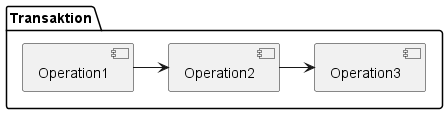
\includegraphics[width=\linewidth]{figures/ChapterSaga/TransactionScopeNormal-0.png}
		\caption{\small Komponentendiagramm Scope einer normalen Transaktion mit 3 Operationen}
		\label{fig:transactionscope-normal}
	\end{minipage}\hspace{\fill}%
	\begin{minipage}{.45\textwidth}
		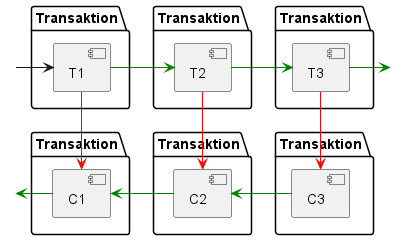
\includegraphics[width=\linewidth]{figures/ChapterSaga/TransactionScopeSaga-0.png}
		\caption{\small Komponentendiagramm Scope einer Saga mit 3 Operationen}
		\label{fig:transactionscope-saga}
	\end{minipage}
\end{figure}
\FloatBarrier

Die Blockierung einer Ressource besteht nur solange, wie sich eine dieser Teiltransaktionen in Ausführung befindet. Nach Beendigung wird die die Teiltransaktion committet. Die Atomarität geht hier also teilweise verloren. Das Gesamtsystem befindet sich zwischen Abschluss von T\textsubscript{1} und Abschluss von T\textsubscript{3} oder C\textsubscript{1} in einem intermediären Zustand, der andere Transaktionen beeinflussen kann. Somit wird auch die Isolation aufgelöst. Dadurch ist es möglich, dass ein inkonsistenter Zustand in das System eingeführt wird. Es werden alle ACID-Eigenschaften außer der Dauerhaftigkeit aufgebrochen.


